\section{Nombre: Ciudadanos} \label{per:ciudadanos}  
\subsection{Descripción:}
Personas comunes de la época prehispánica mesoamericana.
\begin{itemize}
	\item \textbf{Hombre con jarrón:}
	Hombre adulto con solo ropaje cubriendo la parte baja del cuerpo, se encuentra cargando un jarrón con las manos por atrás.
	\item \textbf{Hombre con cacao:}
	Hombre adulto con solo ropaje cubriendo la parte baja del cuerpo, se encuentra cargando un saco de cacao con las manos por atrás.
	\item \textbf{Hombre noble:}
	Hombre adulto con ropaje cubriendo el torax y la parte baja de su cuerpo de colores brillantes.	
	\item \textbf{Mujer con jarrón:}
	Mujer adulta con vestido cargando un jarrón sobre su cabeza.
	\item \textbf{Mujer de puesto:}
	Mujer adulta recostada sobre sus piernas sobre un puesto, que consiste en una manta y sobre de ella algunos artículos de cerámica.	
	\end{itemize} 
\subsection{Status:}
NPC
\subsection{Imagen}
Ver figura \ref{fig:Ciudadanos}.
\begin{figure}
	\centering
	\subfigure[Hombre con jarrón.]{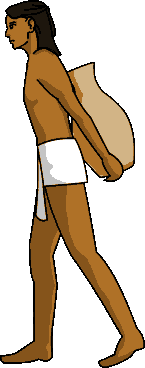
\includegraphics[scale=0.5]{Imagenes/hombre02}}
	\subfigure[Hombre con cacao.]{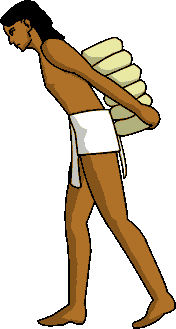
\includegraphics[scale=0.5]{Imagenes/hombre01}}
	\subfigure[Hombre noble.]{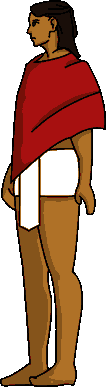
\includegraphics[scale=0.5]{Imagenes/hombre03}}
	\subfigure[Mujer con jarrón.]{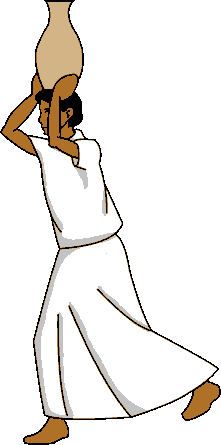
\includegraphics[scale=0.5]{Imagenes/mujer01}}
	\subfigure[Mujer de puesto.]{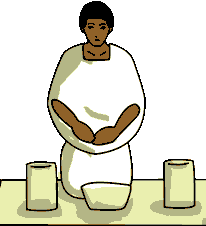
\includegraphics[scale=0.5]{Imagenes/mujer02}}
	\caption{Ciudadanos que se encuentran.}
	\label{fig:Ciudadanos}
\end{figure} 
\subsection{Concepto:}
Los ciudadanos se encuentran para relatar al jugador la época en la que se encuentra, la situación actual que enfrentan, el lugar donde se encuentran y más datos para entender el contexto que lo rodea.
\subsection{Encuentro:}
En el nivel 1.